\documentclass[12pt]{article}

\usepackage{sbc-template}
\usepackage{cite}
\usepackage{graphicx,url}
\usepackage[utf8]{inputenc}
\usepackage[brazil]{babel} 

     
\sloppy

\title{Aplicação de \textit{Automatic Number Plate Recognition} (ANPR) no controle de acesso de veículos}

\author{Maurício de A. Cordeiro\inst{1} }

\address{Instituto Federal de Educação, Ciência e Tecnologia da Bahia\\ 
	Avenida Sérgio Vieira Melo, 3150. Bairro Zabelê - Vitória da Conquista - BA - Brasil\\
	CEP 45078-900
  \email{mauriciocordeiro@live.com}
}

\begin{document} 

\maketitle

\begin{abstract}
  \textit{soon...}
\end{abstract}
     
\begin{resumo} 
 Este trabalho consiste no desenvolvimento de sistema para controle de acesso de veículos baseado em ANPR (\textit{Automatic Number Plate Recognition}), com largo potencial de sua aplicação em locais ou espaços físicos que exigem algum nível de segurança, quando da entrada e saída de pessoas (a título de exemplo, citam-se aqui condomínios e estacionamentos privados). 
\end{resumo}

\section{Introdução}

\subsection{Trabalhos correlatos}


\section{Arquitetura} \label{sec:architecture}

A solução desenvolvida neste trabalho é baseia-se na arquitetura de microsserviços, com módulos conteinerizados, que se comunicam via HTTP, além da aplicação de tecnologias baseadas em ANPR. Esta seção se dedica a detalhar esses conceitos.

\subsection{Arquitetura de Microsserviços}

Arquitetura de Microsserviços (\textit{Microservices Architecture} - MSA) é um modelo arquitetural onde processos de \textit{software} são realizados por componentes fracamente acoplados, que possuem funcionalidades específicas e bem definidas, e que se comunicam através de interfaces padronizadas \cite{viggiato2018}.

A MSA pode ser considerada como a segunda iteração da Arquitetura Orientada a Serviços (\textit{Service Oriented Architecture} - SOA), onde serviços complexos são decompostos em partes mais flexíveis, especializadas e de fácil manutenção, de modo que cada uma é responsável por uma única e pequena funcionalidade com o intuito de realizá-la bem \cite{homay2019}. 

\subsection{Virtualização baseada em contêiner}

A Virtualização baseada em contêiner consiste \cite{eder2016} na utilização de recursos de \textit{hardware} e do \textit{kernel} de um sistema hospedeiro para a criação de ambientes isolados para a execução de determinados processos, o chamado \textbf{contêiner}, esquematizado na Figura~\ref{fig:conteiner}.

\begin{figure}[ht]
	\centering
	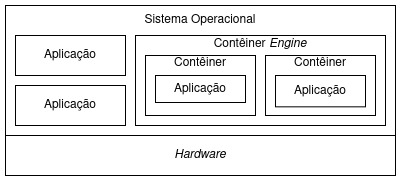
\includegraphics[width=.8\textwidth]{conteiner.jpg}
	\caption{Virtualização baseada em contêiner}
	\label{fig:conteiner}
\end{figure} 

Nessa abordagem, o contêiner aloca apenas os recursos necessário para executar sua aplicação, enquanto trabalha isolado de outros contêineres que possam estar em execução em um mesmo hospedeiro. Essa característica corrobora com sua utilidade quanto a aplicação em soluções baseadas de MSA, uma vez que os contêineres são capazes de se comunicar entre si.


\subsection{REST}

\subsection{ANPR}

\section{"O trabalho"}

\section{Resultados}

\section{Conclusão}

\textit{trabalhos futuros}

\bibliographystyle{sbc}
\bibliography{sbc-template}

\end{document}
